\chapter{Abschluss} \label{abschluss}
\section{Bekannte Fehler}
\subsection{Konfigurationsmenü}
Durch das Konfigurationsmenü kann die Applikation momentan vom einem Benutzer zum abstürzen gebracht werden. Grund dafür ist das komplexere State Management, welches noch nicht 100\% durchgedacht wurde. Mit bestimmten Interaktionen kann ein Fehler auftreten, welcher im momentanen Stand nicht behandelt wird. Dies sorgt so für einen Absturz.
Allerdings wird die Funktionalität der Applikation dadurch nicht beeinträchtigt, da durch das \amk{normale} interagieren der Fehler nicht auftritt.
\subsection{Verlinkung von Assets zu Meshes}
Die automatische und manuelle Verlinkung funktioniert und die Applikation ist nutzbar. Jedoch gibt es einige Edge Cases durch welche auffält, dass die Implementation noch nicht ganz perfekt ist. Grund hierfür ist die darunterliegende Datenstrucktur.

Die Abbildung \ref{fig:db-erweiterung} stellt dar, dass ich in der Vorarbeit die Tabellen \amk{asset}, \amk{product}, \amk{tag} und \amk{status} bereits erstellt habe. Die Priorität war damals, dass alle Daten in die Datenbank übernommen werden und dadurch so wenig Anfragen wie möglich an Netilion gesendet werden. Dazu kommt noch, dass die Schnittstelle für die Assets gleich noch die Informationen der restlichen drei Tabellen mitsenden kann, ohne das man mehrere Requests machen muss. Umgekehrt, also vom Tag zum Asset geht dies nicht.

Durch diese Vorbedingungen/Erfahrungen spielte die Asset Tabelle eine zentrale Rolle im Datenbankschema. Dies stellte sich später allerdings als negativ heraus. Die vorgeschlagene Lösung enthielt eine Hilfstabelle namens \amk{mesh}, womit ein Asset verlinkt werden sollte. Durch diese Implementation ist es nun möglich, dass mehrere Assets des gleichen Modelles mit demselben Mesh verlinkt sind.

Eine bessere Lösung wäre es, wenn der Tag die zentrale Rolle übernehmen würde. Dadurch würde die Hilfstabelle \amk{mesh} nicht mehr verwendet werden müssen. Ausserdem könnte so ein Asset nur mit einem Mesh verlinkt werden, was die Fehleranfälligkeit vermindert.

Dies zu Ändern hätte allerdings den Rahmen einer IPA deutlich gesprengt. Gerne werde ich nach der IPA das ganze genauer analysieren und implementieren.
\section{Verbesserungsmöglichkeiten}
\subsection{Layout verschiebungen}
Es kommt im Frontend momentan sehr oft zu Layout verschiebungen. Damit gemeint ist, dass Elemente, mit dennen der User interagieren möchte, durch State Changes die Position verändern. Aus User Experience Sicht ist dies schlecht gelöst. Beispiel hierfür ist das Vorschlagen von Adressen. Sobald der User einen Teil einer Adresse eingibt, erscheinen drei bis fünf Vorschläge. Diese Vorschläge schieben andere Elemente wie Eingabefelder weiter nach unten.

Dieses Problem kann in React sehr schön und einfach mit dem Drittanbieterpacket \href{https://www.framer.com/motion/}{\code{framer-motion}} gelöst werden. Ich habe bereits Erfahrungen damit gesammelt und würde gerne nach der IPA dies Implementieren.
\subsection{Refresh Token verschlüsseln}
Im Dokument ist erwähnt, dass der \code{refresh\_token} des Benutzers verschlüsselt in der Datenbank gesichert wird. Dies hatte während der Implementierungsphase eine niedrige Priorität, da es nicht direkt zur Funktionalität beitrug. Nun bleibt keine Zeit mehr für die Implementation. Ich werde dies baldmöglichst nach der IPA implementieren, da mir die Sicherheit der Applikation sehr wichtig ist.
\subsection{Unit test/-s}
In der Aufgabenstellung stand, dass die Methode, welche die Assets mit Meshes verlinkt, mit automatischen Tests abgedeckt werden soll. Mit Tests habe ich in Nestjs sehr wenig Erfahung, wodurch mich eine Implementation des Testes einiges an Zeit gekostet hätte. Ich habe dies nun bewusst weggelassen, damit ich mich auf andere Aufgaben fokussieren kann.
\section{Verstösse gegen die Coding Guidelines}
\subsection{Frontend}
\subsubsection{/pages/settings/location.js:19}
\begin{figure}[H]
  \centering
  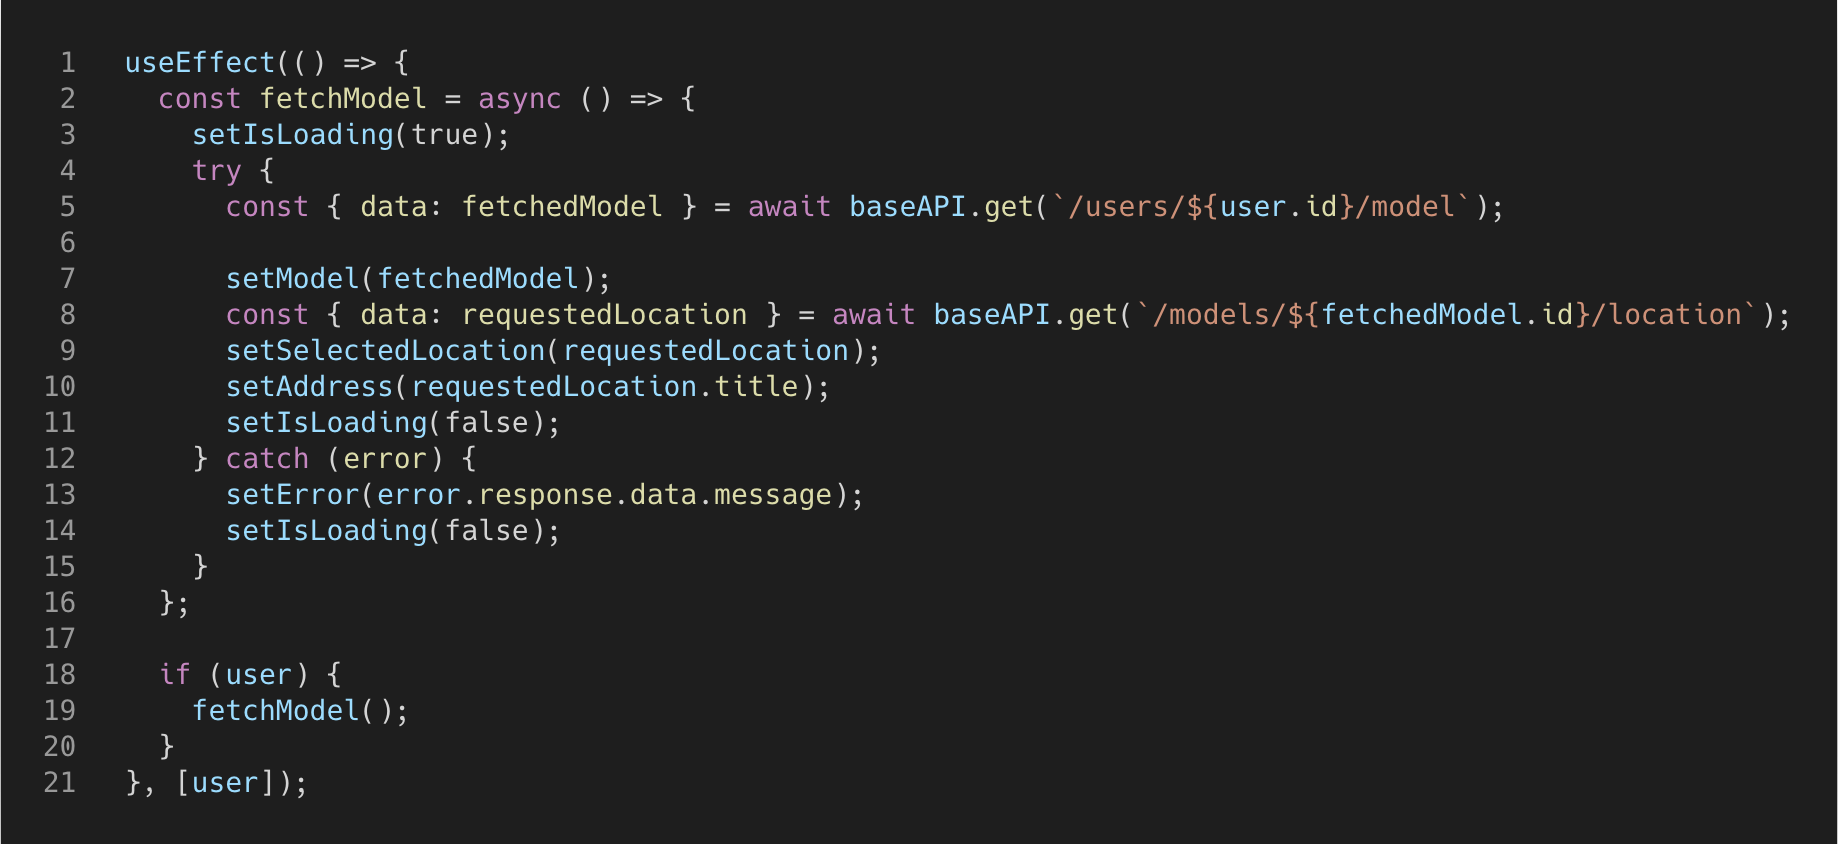
\includegraphics[width=.95\linewidth]{./images/verstoss-1.png}
  \caption[{Abbildung der useEffect Hook in location.js}]{Abbildung der useEffect Hook in location.js}
\end{figure}
Dieser Verstoss ist zu Begründen auf die vielen State updates die innerhalb der useEffect Hook geschehen. Dies ist nicht wirklich sinnvoll auslagbar.
\subsubsection{/pages/settings/model.js:16}
\begin{figure}[H]
  \centering
  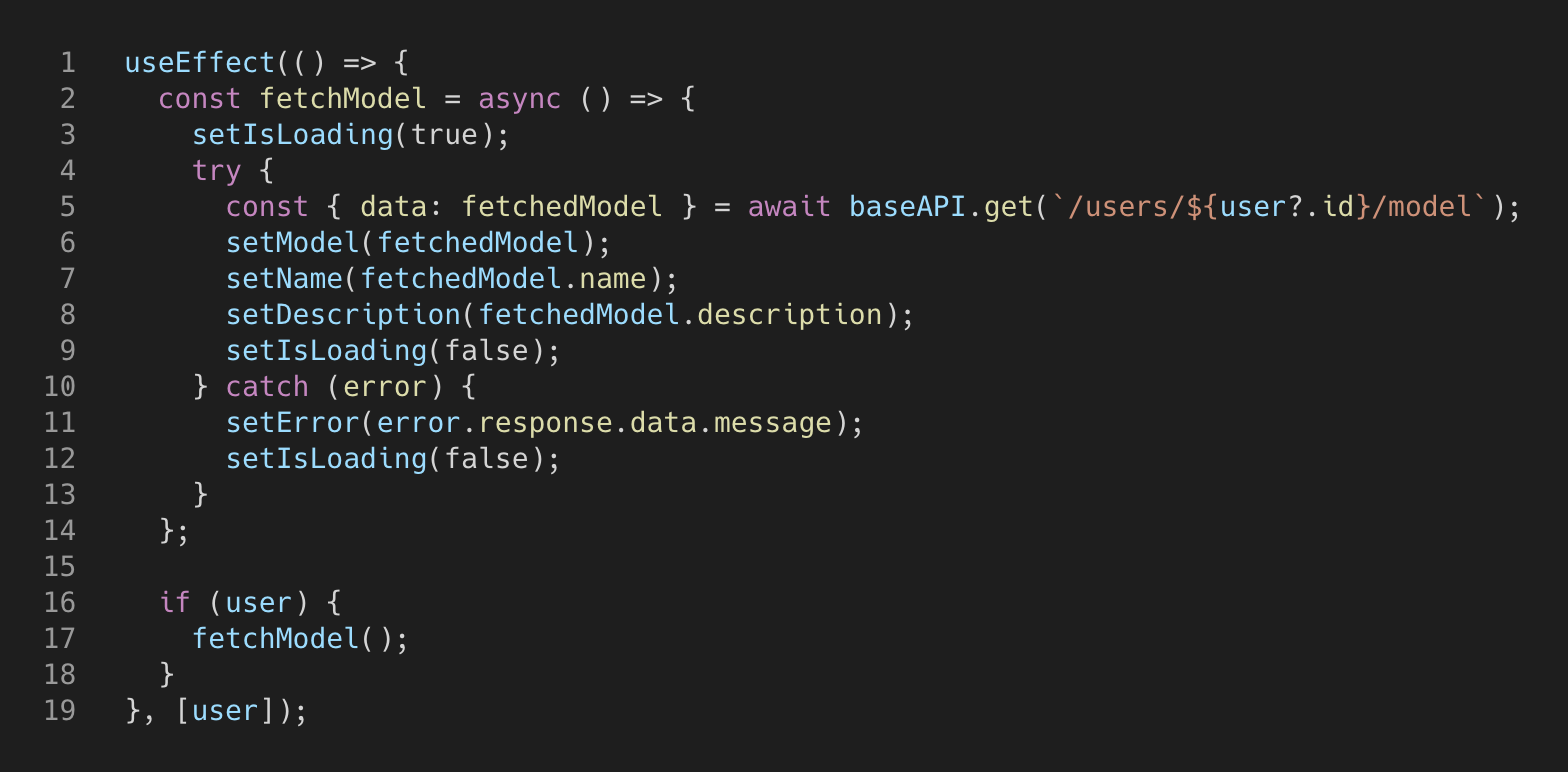
\includegraphics[width=.95\linewidth]{./images/verstoss-2.png}
  \caption[{Abbildung der useEffect Hook in model.js}]{Abbildung der useEffect Hook in model.js}
\end{figure}
Dieser Verstoss folgt der gleich gleichen Begründung wie der erste.
\subsection{Backend}
\subsubsection{/src/netilion-request/netilion-request.service.ts:43}
\begin{figure}[H]
  \centering
  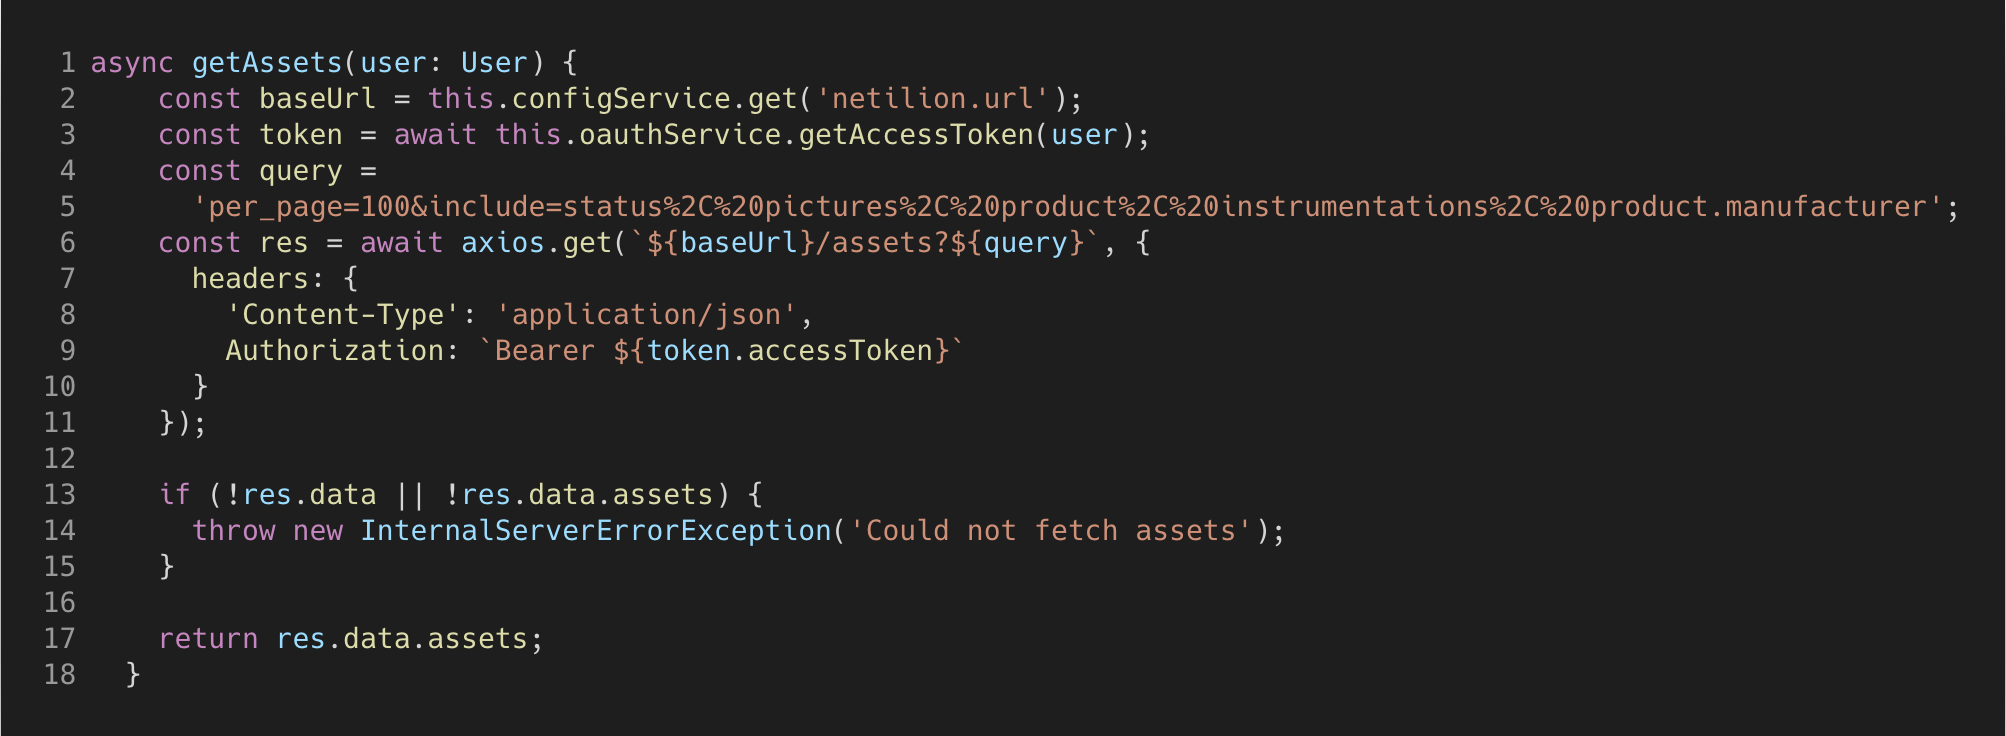
\includegraphics[width=.95\linewidth]{./images/verstoss-3.png}
  \caption[{Abbildung der getAssets Funktion}]{Abbildung der getAssets Funktion}
\end{figure}
Bei dieser Funktion handelt es sich bereits um eine Auslagerung. Jede Zeile muss in dieser Funktion sein und ist sinnlos auszulagern.
\subsubsection{/src/netilion-request/oauth.service.ts:18\&43}
Auch bei diesen Funktionen handelt es sich um ausgelagerte Rest Abfragen. Jegliche Teile auszulagern würde nur den Code schwerer zum Verstehen machen.
\section{Schlussbetrachtung}
\subsection{Reflexion}
Wie man vielleicht den Arbeitsjournalen ablesen konnte, war ich in den vergangen zehn Tagen durchgehend in Stresssituationen. Rückblickend gesehen, hätten wir den Auftrag etwas kürzen können. Ich hatte auch am Anfang der Implementierungsphase extremen Respekt davor, dass ich den Anmeldeprozess mit OAuth2 nicht schaffen werde. Beziehungsweise das es mir viel zu viel Zeit wegnehmen könnte, sodass ich folglich zu wenig Zeit für andere Aufgaben hätte. Dies ist zum Glück nicht aufgetreten und es verlief alles recht positiv.
\subsection{Schlusswort}
Ich konnte mit dieser Arbeit eine grosse Erweiterung des OSE-Dashboards erstellen. Diese kann nun von verschiedenen Endress+Hauser Standorten eingesetzt werden, um den Kunden die Möglichkeiten von Netilion Connect näher zu bringen.
\subsection{Persönliche Bilanz}
Ich bin mir sicher, dass ich einige Erfahrungen dieser Arbeit in mein weiteres Berufsleben mitnehmen kann. Ich konnte unter Druck arbeiten, wobei meine Leistung in den ganzen zehn Tagen nicht abgenommen hat. Ich hatte viele Momente in diesen Tagen, an dennen ich am liebsten einfach nichts gemacht hätte für ein bis zwei Stunden, da ich so unter Druck stand. Jedoch habe ich es durchgezogen und merkte dadurch, dass dies nur eine kleine gedankliche Barrier war, die ich überweltigen konnte.
Abgesehen davon investierte ich sehr viel Zeit in diese Technische Dokumentation. Ich denke auch hier, dass mir gewisse Erfahrungen und Eindrücke bleiben werden.
Ausserdem habe ich mit dieser Arbeit eine nahezu perfekte Implementation von OAuth2 im Bezug auf den Anmeldeprozess erstellt.

Ich bin mehr als nur zufrieden mit meinen erreichten Ergebnissen.